\fancychapter{Introduction}
\cleardoublepage
\label{chapter:1}

\section{Context}
% What is language and speech
The faculty of expressing or describing thoughts, feelings and needs by using language is a fundamental capability in our daily lives. As per by the Oxford dictionary,  \textit{language is defined as the system of communication in speech and writing that is used by people of a particular country or area}. Consequently, language can be conceptualised as an intricate and rule-governed system that empowers individuals to convey abstract concepts, share experiences, and take part in nuanced forms of communication. Effective communication through language begins with the conceptualisation of the message to be transmitted (\textit{conceptualisation}), followed by the selection of appropriate lexical items and subsequent grammatical encoding, culminating in their meaningful organisation (\textit{formulation}). Subsequently, the linguistic representation is transformed into sound through the transmission of this representation from the brain to the muscles of the complex speech system including lips, larynx, glottis, lungs, jaw and tongue (\textit{articulation}) \cite{levelt1993speaking}. Unlike language, which encompasses both spoken and written forms, speech specifically refers to the spoken manifestation of language.


% Children speech and language acquisition
The capability to speak and comprehend language is not inherently present but rather develops gradually over time with experience. Babies instinctively engage in pre-linguistic communication, using gestures, facial expressions, and vocalisations to articulate their basic needs. As language acquisition progresses, children transition to the babbling stage, experimenting with sound patterns. Eventually, speech emerges, marking a crucial milestone in communication development, and typically, children reach specific language milestones at particular ages. For example, around 12 to 18 months, a child usually utters their first words and starts imitating sounds. By the age of 4 to 5, children tend to formulate sentences and grasp more intricate concepts. Regarding speech sounds, younger children, approximately 1 year old, can produce basic speech sounds like \textit{/p/}, \textit{/b/}, \textit{/m/} while older children, around 5 years old, can articulate more complex sounds such as \textit{/r/} and \textit{/th/}. This developmental stage is referred to as language acquisition, and it plays a crucial role in a child's overall development. Indeed, our daily dependence on social and communication skills endures throughout our entire lives. Consequently, it is imperative for children to develop the capacity to interact effectively with others to achieve seamless integration into society across all aspects of their lives.

% But pathology exists, need for therapy/assessment
Regrettably, a subset of children experience speech disorders stemming from congenital conditions such as cleft palate, cerebral palsy, and prelingual deafness. Alternatively, certain individuals may acquire speech-related issues during childhood, encompassing cognitive developmental delays, breathing-feeding-swallowing disorders and traumatic brain injuries. Notably, in 2012, empirical data \cite{black2015communication} highlighted that 7.7\% of children aged 3 to 17 in the United States of America exhibited communication disorders, with 5.0\% of this cohort specifically presenting speech-related problems.

Furthermore, findings \cite{langbecker2020long} suggest that individuals with childhood speech disorders may confront an increased prevalence of mental health challenges, diminished social well-being, and reduced academic accomplishments in comparison to their healthy peers. This highlights the complex nature of speech disorders in children, the consequences of which extend into adolescence and adulthood. Hence, early identification and intervention play a pivotal role in mitigating the enduring effects on these children's social interactions, society integration, communication skills, educational progress, and overall well-being.

% Speech therapy
Pediatric \acp{SLP} play a crucial role in providing therapy to help children overcome the effects of speech disorders and offer early diagnosis. The therapy typically includes exercises and assessments, which can be based on perceptual speech evaluations or standardised tests. To effectively engage children, these activities are often presented as games, taking into consideration the inherently limited attention span of children. Notably, \acp{SLP} frequently maintain long-term follow-ups with their patients, allowing them to monitor the evolution of speech quality over time and personalise exercises to the specific needs of each child. The adoption of this individualised therapeutic approach is essential for helping children achieve improved speech and communication skills.

% Problems with speech therapy (hospital, stress, ...)
However, a prominent challenge arises concerning the accessibility and availability of speech therapy services. Numerous children, particularly those residing in underserved or remote areas, encounter obstacles in accessing speech therapy resources. Additionally, the hospital environment introduces an additional layer of stress for children. While clinically necessary, therapeutic settings may inadvertently contribute to heightened anxiety and discomfort, as children may perceive it as intimidating. Furthermore, the logistical challenges associated with frequent hospital visits impose a substantial financial and time burden on families.

Another obstacle pertains to the continuity and consistency of therapy. Children may experience interruptions in their therapeutic journey due to factors such as financial constraints, scheduling conflicts, or alterations in healthcare coverage. These disruptions have the potential to impede progress and undermine the effectiveness of the therapy. Lastly, it is imperative to acknowledge that, despite professional training, inter-expert variability in perceptual assessments may persist, resulting in disparate diagnostic conclusions. To address these challenges, adopting a hybrid approach that combines in-person therapy with technology holds potential benefits \cite{hilty2015new,barnett2011utilizing}. Teletherapy, for instance, has emerged as a promising avenue to bridge geographical gaps and deliver therapy services remotely \cite{hughes2019increasing}.

\begin{figure}
    \centering
    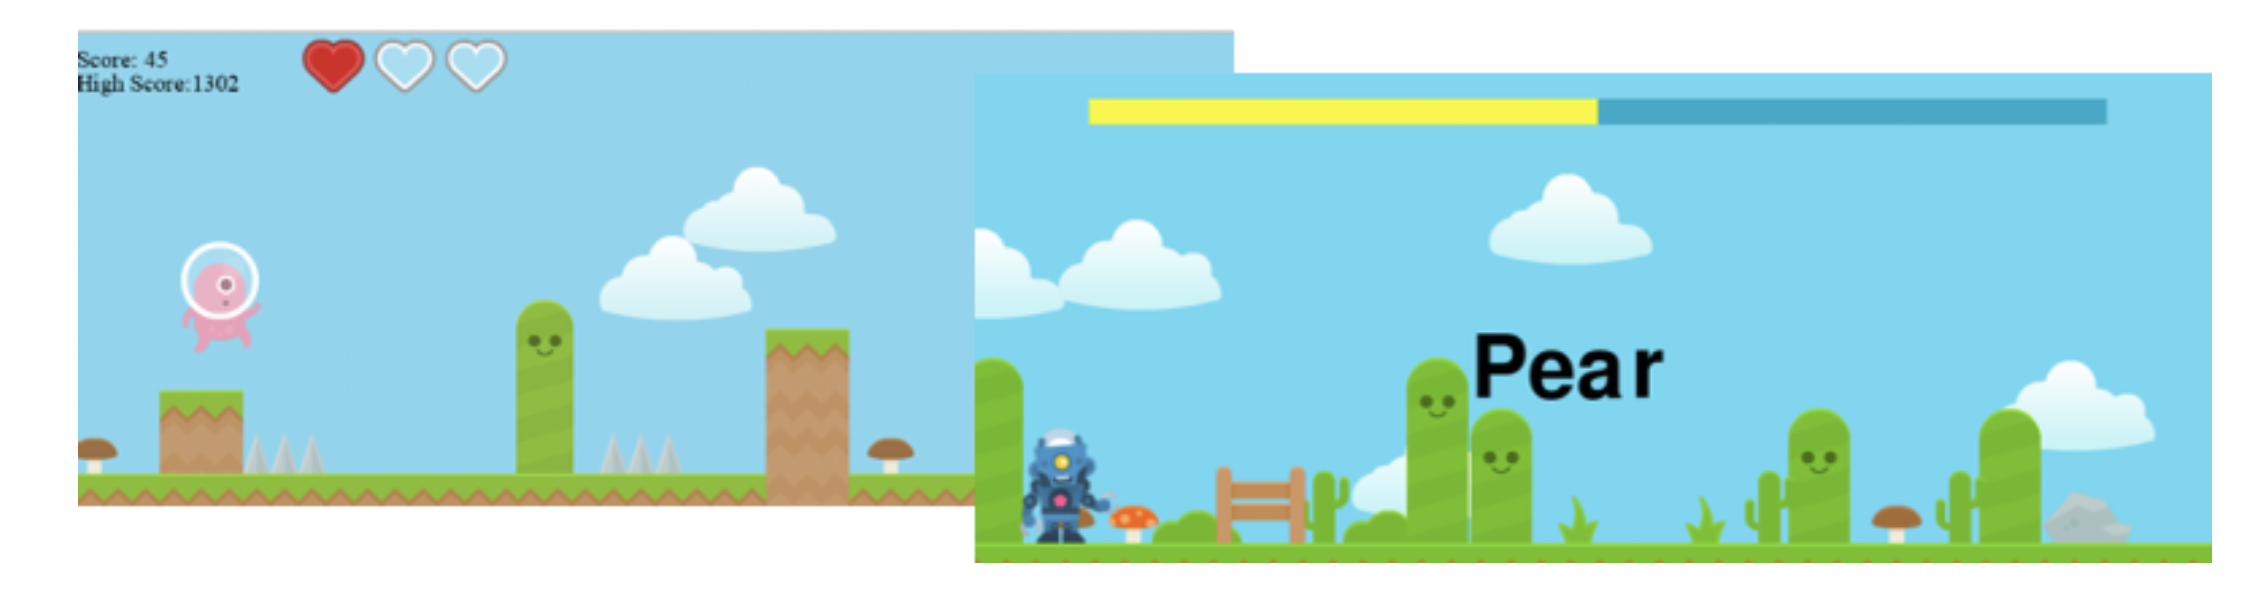
\includegraphics[width=1\textwidth]{imgs/exampleSLT.png}
    \caption{Illustrated herein are some examples of children's Speech and Language Technology applications that were developed during the course of this thesis. On the left is a running platformer game, where the user's voice controls the character. Pitch dictates running and jumping actions, while energy modulates the velocity of these actions. On the right, a reading task game is depicted, wherein a robot instructs the user to read designated words.}
    \label{fig:exSLT}

\end{figure}

% SLT could be the beginning of the answer and is already used in real life
In this context, \ac{SLT} have emerged as highly pertinent within the domain of speech therapy \cite{mendoza2022added}. These technologies encompass a spectrum of computational tools designed to analyse, understand and provide objective and precise automated assessments. Another benefit lies in their potential integration into gamification frameworks, thereby augmenting children's involvement during therapy \cite{brewer2013using}. Moreover, the ability to record speech utter by the patient during a session using \ac{SLT} enables post-session thorough analysis and long-term monitoring by the therapist. Due to the aforementioned reasons, the development of such tools has gained considerable attention, empowering patients to engage in exercises beyond therapy sessions, notably in a home setting. Several \ac{SLT} examples developed within the scope of this thesis are illustrated in Figure \ref{fig:exSLT}.

\section{Problem statement}
% Technologies are more and more present
Recent years have seen increased integration of \ac{SLT} into various aspects of our daily lives, impacting a wide range of environments, including homes, transportation, education, and even the military. Noteworthy examples encompass voice assistants, hands-free computing, healthcare systems, automatic helplines, and speech-to-speech translation services. The performance progress in these applications was made possible through the use of machine learning techniques, especially deep learning approaches, the increasing computational capacities of our devices, and the ever-growing volume of data available to train and improve these systems.

% Children are a good target audience for SLT
Children represent a promising target audience for \ac{SLT} due to the inherent complexities of conventional computer interfaces, which pose challenges for them and limit their capacity to fully benefit from digital platforms. Indeed, children commonly face difficulties in manipulating mouse and keyboard inputs. Additionally, the abstract nature of traditional man-machine interfaces can impede the understanding necessary for effective interaction. In this context, speech-based systems emerge as a promising alternative, offering a more natural and accessible means for children to interact with technology. Through the use of speech recognition technologies, these speech systems mitigate the barriers associated with conventional interfaces, providing a fluid and intuitive interaction paradigm that aligns more closely with the developmental stages and cognitive abilities of young users. Another potential application of \ac{SLT} for children could be in the development of automatic reading tutors. Given that the process of learning to read is individual and varies for each child, a personalised automatic reading tutor could assist in tailoring the learning experience to the specific needs of each student. This has the potential to reduce the workload on teachers and provide additional support in the crucial skill of reading acquisition. Finally, the growing presence of voice assistants in home settings underscores the importance of reliable \ac{ASR} for children. In this context, a reliable ASR system becomes crucial to ensure a positive and effective user experience of seamless interaction with voice-enabled devices in various home environments.

% Automatic tools for speech therapy
As previously mentioned, \ac{SLT} applications are gradually making their way into the field of atypical speech, particularly for children. While these automatic tools are currently in their early stages and have limitations, there is indeed a rising interest in implementing atypical speech and language therapy systems with a focus on assisting \acp{SLP}. In this context, systems capable of automatically recognising speech content, assessing pronunciation quality and automatically detecting speech pathologies could be highly valuable in supporting pediatric \acp{SLP} and patients.

All of these objectives require the implementation of a robust \ac{ASR} system specifically tailored for healthy children, serving as a foundational model. Nevertheless, while speech recognition technologies for adult speakers have made substantial advancements, leading to increased accuracy, the performance of \ac{ASR} systems for children remains underperforming in comparison. This discrepancy results in unreliable systems for children and, by extension, their use in \ac{SLT} applications. This diminished performances can be attributed to a combination of factors, including intra- and inter-speaker variability, limited linguistic and phonetic knowledge, and the scarcity of available data.

% In this work we propose....
In this thesis, we will undertake a comprehensive investigation into the intricacies of children's speech, closely examining the inherent differences between children and adults in the domain of \ac{ASR}. Through this examination, the objective is to analyse the constraints associated with the application of adult-based systems to children's speech and, subsequently, to outline the methodologies present in the literature for enhancing \ac{ASR} systems. The overarching goal of this thesis is to establish a robust foundational system that effectively addresses the recognition of children's speech.

% Explain that there is no Pathological speech dataset
Initially, the context of this thesis aimed at addressing pathological speech for children. However, due to constraints in data availability, specifically the absence of a meaningful pathological children's speech dataset, experiments related to pathological speech in children were not included in this thesis. 
The shift in focus towards improving \ac{ASR} for healthy children was motivated by the importance of establishing a solid \ac{ASR} foundational system focusing on children. This shift broadens the potential applications of our research, ranging from personal assistants, automatic reading tutors and voice interactions with computer interfaces. Despite the pivot towards healthy children's speech, this thesis encompasses an investigation into adult pathological speech detection, as detailed in Annex \ref{chapter:appendixA}.


% Research question
Our work specifically aims to answer the following research questions:
\begin{enumerate} 
\item Which knowledge transfer approach is best for efficiently modelling and improving automatic recognition of children's speech? Can these approaches be used to efficiently exploit low-resource children's speech data from multiple languages?
\item  How do end-to-end automatic speech recognition models achieve state-of-the-art results for children's \ac{ASR} when finetuned from an adult model? Particularly, what are the components that are most important to fine-tune?
\item Is it possible to develop a parameter-efficient automatic speech recognition model for children? Can we further improve the parameter efficiency with other architectures? 
\item Is it possible to use children's synthetic speech to extend the amount of children's data? How can we control the quality and speakers’ variability?
\end{enumerate}

\section{Contributions}
% State of the art exploration
This thesis commenced with a comprehensive exploration of the current state-of-the-art in children's Automatic Speech Recognition (\ac{ASR}). We present an examination of the fundamental determinants that contribute to the decline in \ac{ASR} performance for children's speech. Additionally, we meticulously assess current research on children's speech. The primary aim was to identify potential avenues for improvement throughout the course of this thesis. 

%HMM-DNN contribution
Subsequent to the literature review, we start our research by the implementation of \ac{HMM-DNN} models for children \ac{ASR}. We explored different strategies to reduce the gap observed between children and adults in the context of both English and European Portuguese speech. We identified the effectiveness of knowledge transfer methods, specifically, transfer learning and multi-task learning. Transfer learning adapts speech recognition adult models by fine-tuning their weights for children's speech. On the other hand, multi-task learning exposed models to both adult and children's speech datasets simultaneously during training. In an innovative synthesis, we proposed to combine transfer learning and multi-task learning into a unified approach, the multi-task transfer learning framework. We applied this approach to multiple low-resource children's datasets from diverse language sources resulted in a publication at LREC 2022:
\begin{itemize}
    \item \textbf{Rolland, Thomas}, Alberto Abad, Catia Cucchiarini, and Helmer Strik. "Multilingual Transfer Learning for Children Automatic Speech Recognition." \textit{ Language Resources and Evaluation Conference} (2022).
\end{itemize}

% End-to-End contribution
Thereafter, our research turned into the end-to-end paradigm, motivated by the encouraging improvements observed in the end-to-end children's \ac{ASR} performance. We introduced a novel detailed transfer learning approach, called Partial fine-tuning, where our objective was to gain a thorough understanding of the specific components within the end-to-end architecture that significantly contributed to the remarkable improvements in recognition scores. The identification of the most relevant components allowed the development of specific algorithms aimed at further improving the model's recognition performances. Particularly, we explored the integration of an additional set of parameters, the Adapters, directly into the original \ac{ASR} model. This integration facilitated a parameter-efficient approach to adapt the model, accepted at ICASSP 2024:

\begin{itemize}
    \item \textbf{Rolland Thomas} and Alberto Abad. "Exploring adapters with conformers for children’s automatic speech recognition." \textit{ International Conference on Acoustics, Speech and Signal Processing} (2024).
\end{itemize}

% TTS contribution
In response to the scarcity of large children's speech datasets, we delved into the exploration of leveraging synthetic speech to augment the existing dataset. However, our investigation revealed that a mismatch between real and synthetic data hindered the results. To address this challenge, we introduced additional processing steps to efficiently incorporate synthetic data. We proposed a double-way approach, wherein the synthetic data underwent an additional set of parameters. This innovative methodology contributed to an enhanced \ac{ASR} system tailored for children and was published at ICASSP 2024:

\begin{itemize}
    \item \textbf{Rolland Thomas} and Alberto Abad. "Improved children’s automatic speech recognition combining adapters and synthetic data augmentation." \textit{International Conference on Acoustics, Speech and Signal Processing} (2024).
\end{itemize}

% Pathology dectection contributation
In tandem with the primary focus of enhancing children's \ac{ASR}, this thesis extends its scope to the detection of pathologies directly from speech. This secondary investigation retains relevance within the broader context of the thesis, particularly as we initially aimed to address the specific needs of children with pathological speech. We explored the use of embedding extracted from pre-trained models for the detection of different pathologies such as Alzheimer's disease, Parkinson's disease, obstructive sleep apnea and COVID-19:

\begin{itemize}
    \item Anna Pompili, \textbf{Thomas Rolland}, and Alberto Abad. "The INESC-ID multi-modal system for the ADReSS 2020 challenge." \textit{Interspeech} (2020).
    \item Catarina Botelho, Francisco Teixeira, \textbf{Thomas Rolland}, Alberto Abad, and Isabel Trancoso. "Pathological speech detection using x-vector embeddings." \textit{arXiv preprint} arXiv:2003.00864 (2020).
    \item Rubén Solera-Ureña, Catarina Botelho, Francisco Teixeira, \textbf{Thomas Rolland}, Alberto Abad, and Isabel Trancoso. "Transfer Learning-Based Cough Representations for Automatic Detection of COVID-19." \textit{Interspeech} (2021).
\end{itemize}


\section{Structure for the thesis}
The structure of this thesis comprises eight chapters. In Chapter \ref{chap:Chapter2}, we first establish the context of the thesis and understand the challenges associated with automatic children's speech recognition. This chapter also provides an overview of the automatic speech recognition systems, along with an examination of the latest approaches specifically tailored to address the unique challenges posed by children's \ac{ASR}. Furthermore, a compilation of children's speech corpora is presented.

Following, in Chapter \ref{chap:Chapter3}, we present our work on the hybrid speech recognition paradigm, focusing on the evaluation of different knowledge transfer approaches and their combinations. In Chapter \ref{chap:4}, we shift towards the end-to-end paradigm, evaluating the role of the different components of the \ac{ASR} model during transfer learning and proposing our partial fine-tuning procedure. Subsequently, in Chapter \ref{chap:5}, we validate the use of Adapters as a parameter-efficient knowledge transfer approach for children's \ac{ASR}. In Chapter \ref{chap:6}, we build upon this knowledge to propose a novel approach to use imperfect synthetic data as data augmentation during transfer learning.
Next, in Chapter \ref{chap:7}, we investigate possible alternative approaches for parameter-efficient transfer learning, introducing a novel method using a shared Adapter across the different layers of the model. Finally, in Chapter \ref{chap:8}, we conclude the thesis with a summary of the different works and results studied in this thesis, as well as some perspectives of future work. 